%%%%%%%%%%%%%%%%%%%%%%%%%%%%%%%%%%%%
\subsection{Monitoring site exposures v. subjects LHEM results}
\label{subsec:background_monitoring_v_lhem}
%%%%%%%%%%%%%%%%%%%%%%%%%%%%%%%%%%%%

Figures \ref{fig:monitoring_v_lhem_nox_hist} and \ref{fig:monitoring_v_lhem_pm25_hist} show histogram plots of exposure taken from a background monitoring site and a roadside monitoring site (outlined in Section \ref{sec:monitoring_site_data}), compared to exposure using the LHEM, for NO$_{X}$ and PM$_{2.5}$ respectively.

\begin{figure}[H]
\centering
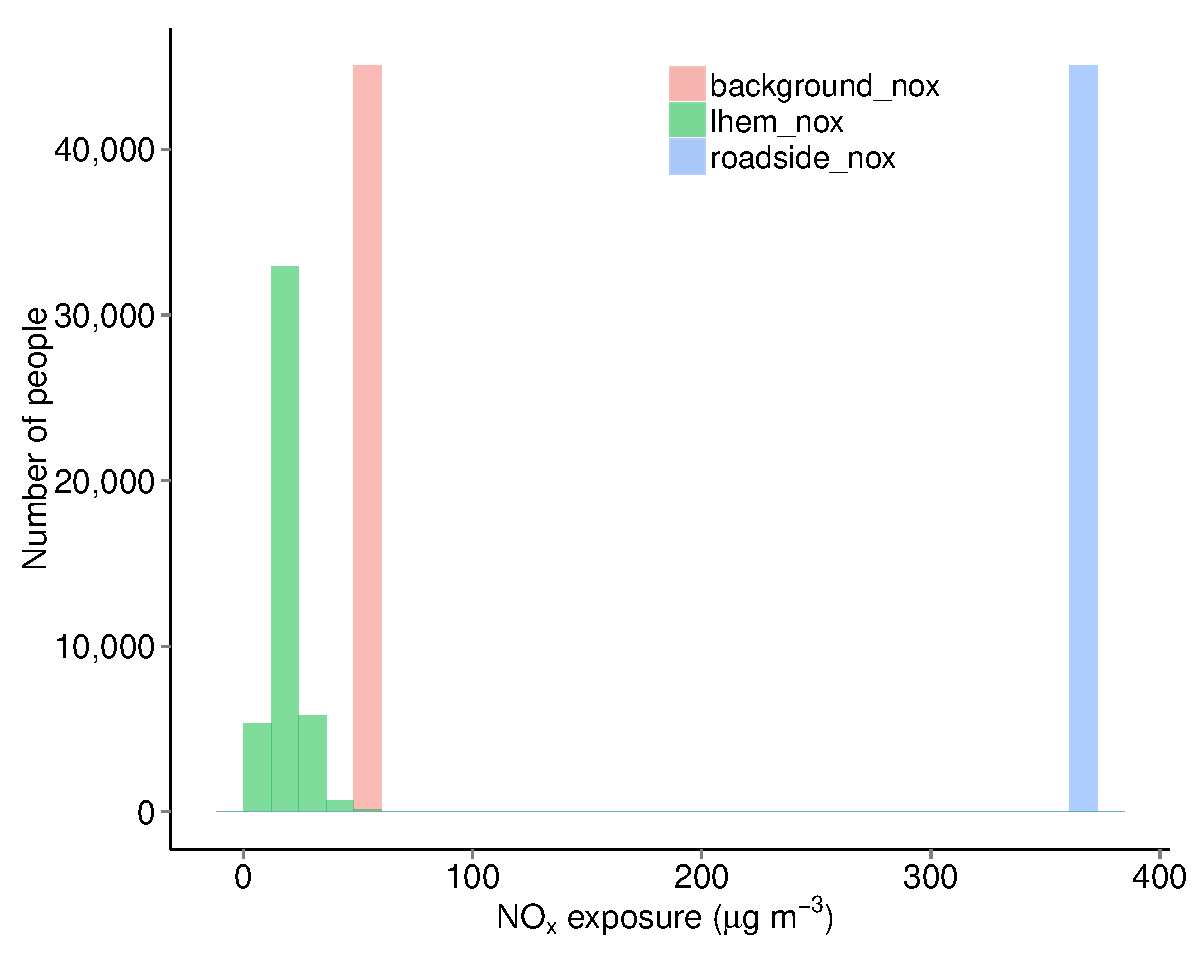
\includegraphics[scale=0.6]{monitoring_v_lhem_nox_hist}
\caption{Daily mean exposure to NO$_{X}$ comparing a background monitoring site, a roadside monitoring side, and exposure with the LHEM}
\label{fig:monitoring_v_lhem_nox_hist}
\end{figure}

\begin{figure}[H]
\centering
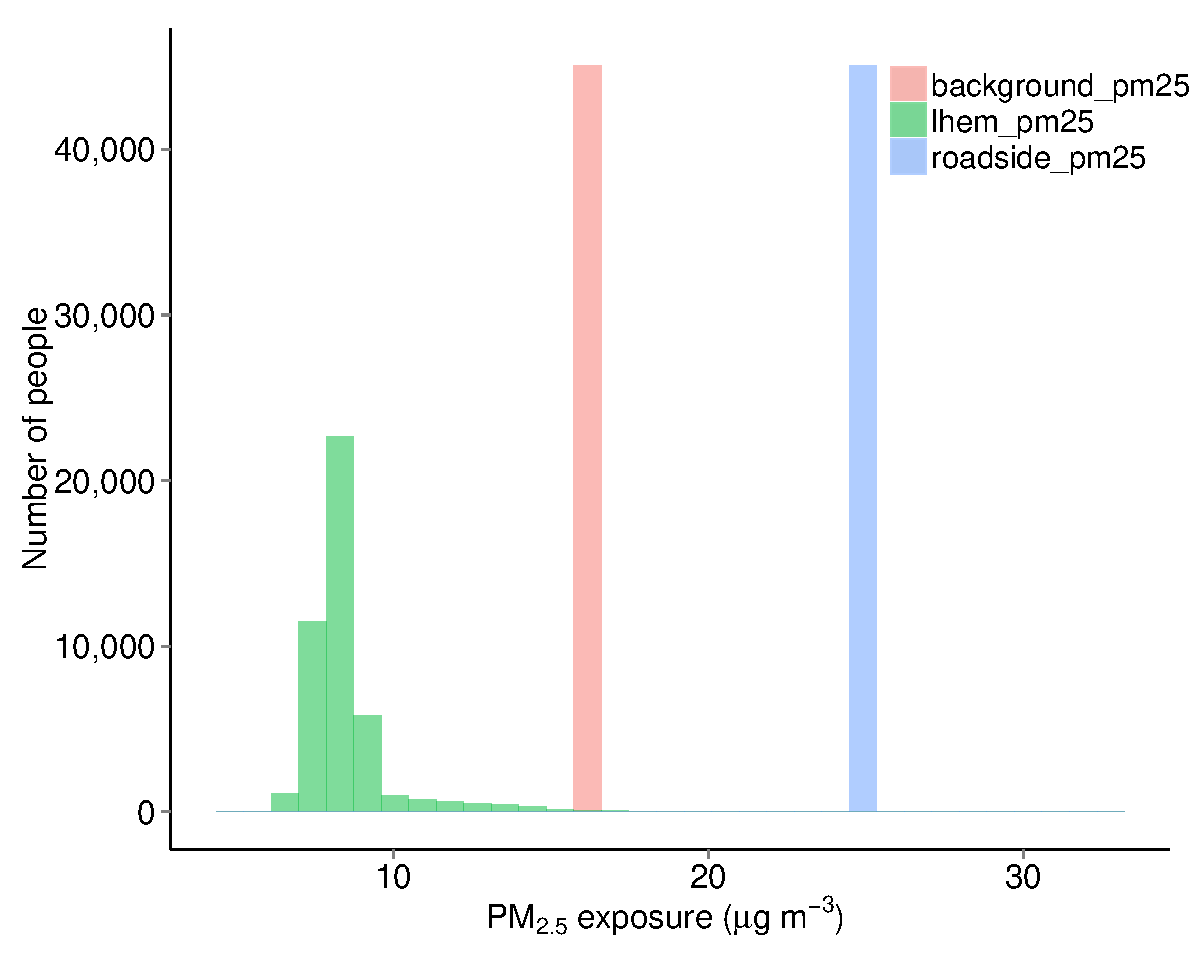
\includegraphics[scale=0.6]{monitoring_v_lhem_pm25_hist}
\caption{Daily mean exposure to PM$_{2.5}$ comparing a background monitoring site, a roadside monitoring side, and exposure with the LHEM}
\label{fig:monitoring_v_lhem_pm25_hist}
\end{figure}

Using the LHEM model the exposure of the population is found to be generally lower than exposure estimates based on a roadside or a background monitoring site.

For NO$_{X}$ the LHEM mean is 18.39 $\mu \text{g m}^{-3}$ and the median is 17.03 $\mu \text{g m}^{-3}$, compared to an annual average value of NO$_{X}$ at the background monitoring site 56.6 $\mu \text{g m}^{-3}$ and 365.41 $\mu \text{g m}^{-3}$ at the roadside site.

For PM$_{2.5}$ the LHEM mean is 8.49 $\mu \text{g m}^{-3}$ and the median is 8.23 $\mu \text{g m}^{-3}$, compared to an annual average value of PM$_{2.5}$ at the background monitoring site of 16.28 $\mu \text{g m}^{-3}$ and 24.60 $\mu \text{g m}^{-3}$ at the roadside site.

Whereas the LHEM results have a range of exposures, the monitoring sites exposure values do not.

The 10th to 90th percentile range for NO$_{X}$ using the LHEM is 11.64 $\mu \text{g m}^{-3}$ to 26.26 $\mu \text{g m}^{-3}$ (a range of 14.62 $\mu \text{g m}^{-3}$), and for PM$_{2.5}$ the LHEM has a 10th to 90th percentile range of 7.32 $\mu \text{g m}^{-3}$ to 9.4 $\mu \text{g m}^{-3}$ (a range of 2.08 $\mu \text{g m}^{-3}$).

%%%%%%%%%%%%%%%%%%%%%%%%%%%%%%%%%%%%
\subsection{Subjects postcode exposure v. subjects LHEM results}
\label{subsec:postcode_v_lhem}
%%%%%%%%%%%%%%%%%%%%%%%%%%%%%%%%%%%%

Figures \ref{fig:postcode_v_lhem_nox_hist} and \ref{fig:postcode_v_lhem_pm25_hist} show histogram plots of exposure at the postcode-level, compared to exposure using the LHEM, for NO$_{X}$ and PM$_{2.5}$ respectively.

\begin{figure}[H]
\centering
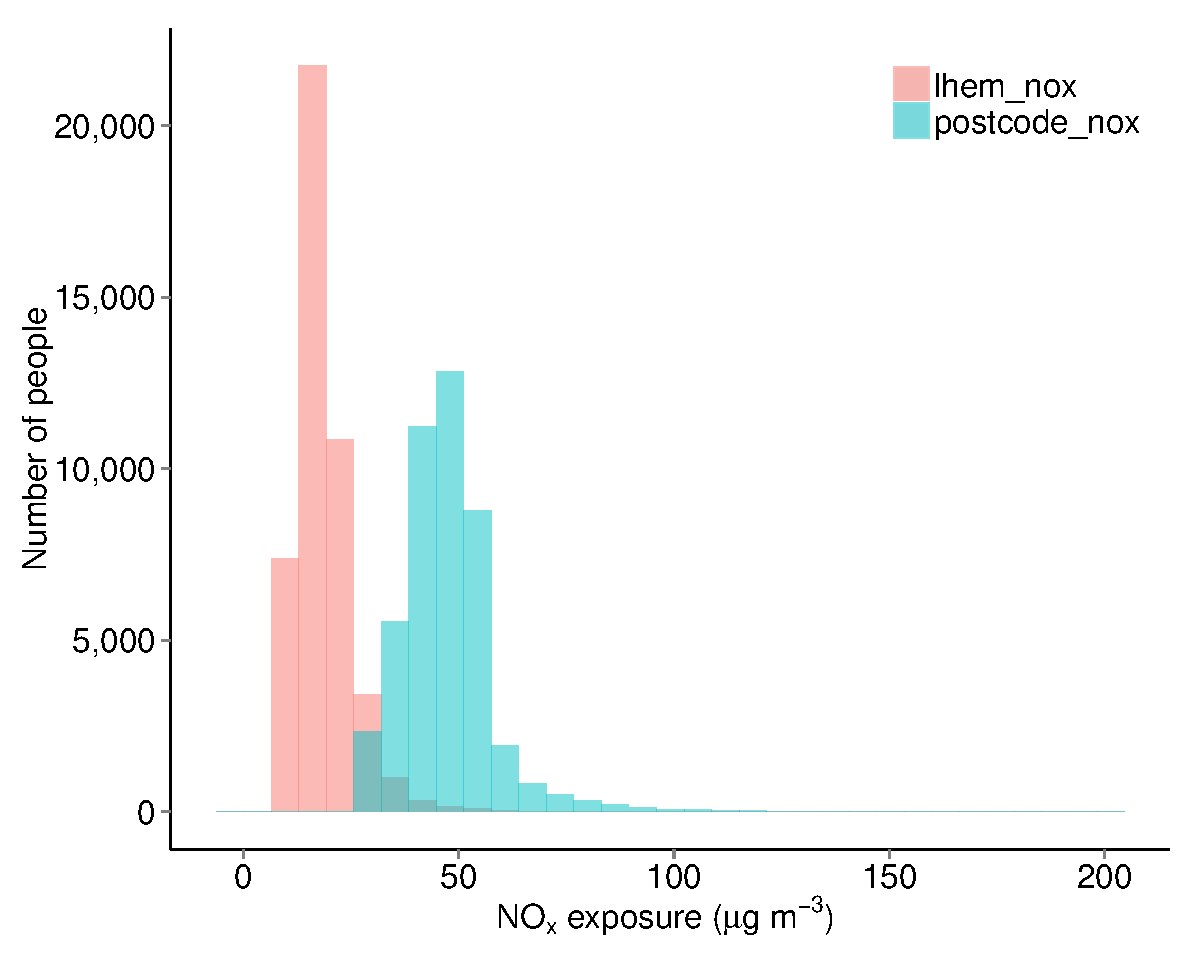
\includegraphics[scale=0.6]{postcode_v_lhem_nox_hist}
\caption{Daily mean exposure to NO$_{X}$ comparing postcode exposure with the LHEM}
\label{fig:postcode_v_lhem_nox_hist}
\end{figure}

\begin{figure}[H]
\centering
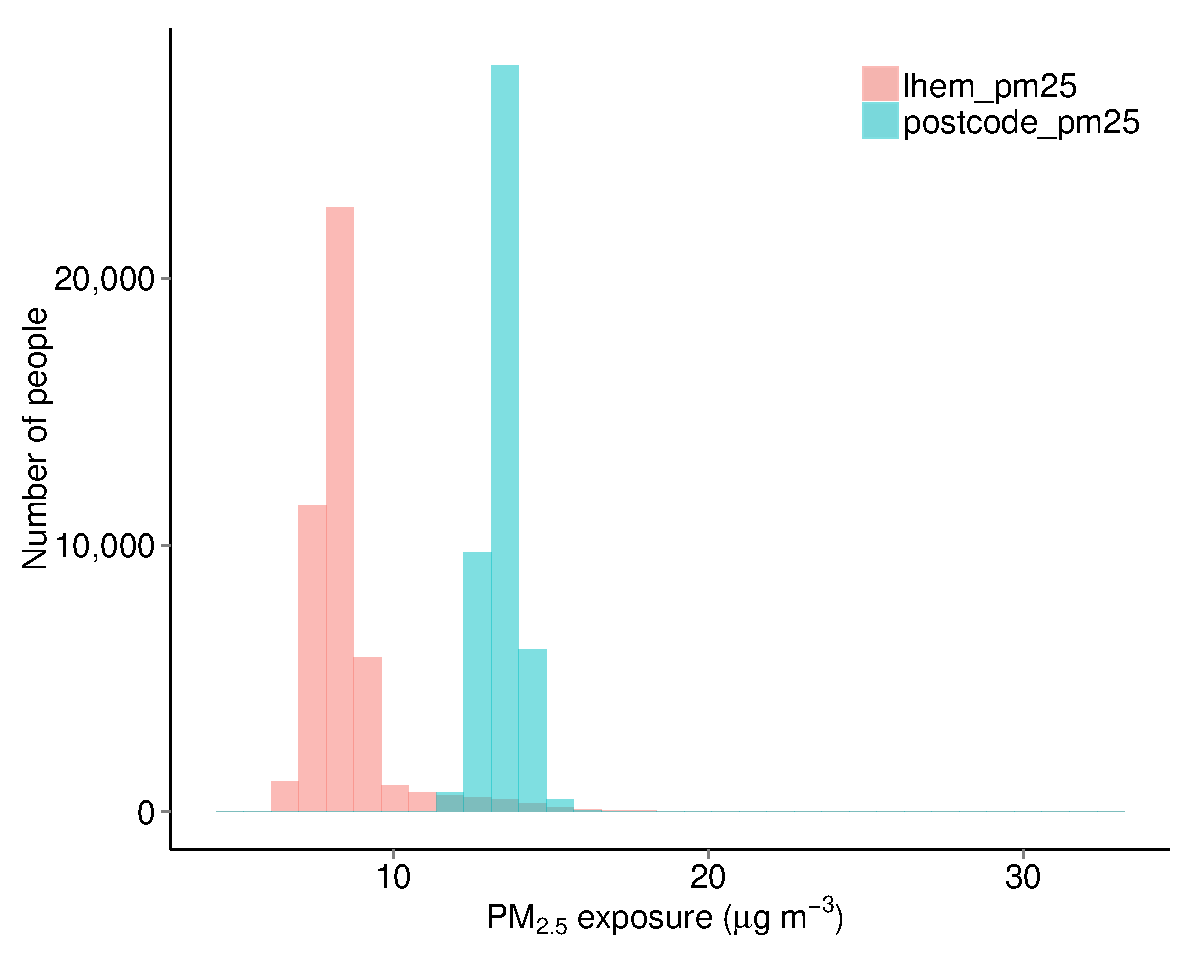
\includegraphics[scale=0.6]{postcode_v_lhem_pm25_hist}
\caption{Daily mean exposure to PM$_{2.5}$ comparing postcode exposure with the LHEM}
\label{fig:postcode_v_lhem_pm25_hist}
\end{figure}

Using the LHEM model the exposure of the population is found to be generally lower than estimates based on the residents postcode.

For NO$_{X}$ the LHEM mean is 18.39 $\mu \text{g m}^{-3}$ and the median is 17.03 $\mu \text{g m}^{-3}$, compared to NO$_{X}$ at the postcode of 47.23 $\mu \text{g m}^{-3}$ and 46.52 $\mu \text{g m}^{-3}$ respectively.

For PM$_{2.5}$ the LHEM mean is 8.49 $\mu \text{g m}^{-3}$ and the median is 8.23 $\mu \text{g m}^{-3}$, compared to PM$_{2.5}$ at the postcode of 13.47 $\mu \text{g m}^{-3}$ and 13.50 $\mu \text{g m}^{-3}$ respectively.

In addition to the LHEM finding different mean and medians to postcode based exposure estimates, I also found different ranges.

The 10th to 90th percentile range for NO$_{X}$ using the LHEM is 11.64 $\mu \text{g m}^{-3}$ to 26.26 $\mu \text{g m}^{-3}$ (a range of 14.62 $\mu \text{g m}^{-3}$), compared to similar percentile ranges for NO$_{X}$ at the postcode of 35.36 $\mu \text{g m}^{-3}$ to 57.18 $\mu \text{g m}^{-3}$ (a range of 21.82 $\mu \text{g m}^{-3}$). That is, we find a smaller range of exposures to NO$_{X}$ using the LHEM than using postcode methods.

For PM$_{2.5}$ the LHEM has a 10th to 90th percentile range of 7.32 $\mu \text{g m}^{-3}$ to 9.4 $\mu \text{g m}^{-3}$ (a range of 2.08 $\mu \text{g m}^{-3}$), compared to similar percentile ranges for PM$_{2.5}$ at the postcode of 12.73 $\mu \text{g m}^{-3}$ to 14.07 $\mu \text{g m}^{-3}$ (a range of 1.34 $\mu \text{g m}^{-3}$). In brief, the range for PM$_{2.5}$ between the LHEM and postcode is similar.

%%%%%%%%%%%%%%%%%%%%%%%%%%%%%%%%%%%%
\subsection{Subjects address-point exposure v. subjects LHEM results}
\label{subsec:address_point_v_lhem}
%%%%%%%%%%%%%%%%%%%%%%%%%%%%%%%%%%%%

Figures \ref{fig:address_point_v_lhem_nox_hist} and \ref{fig:address_point_v_lhem_pm25_hist} show histogram plots of exposure at the address-point, compared to exposure using the LHEM, for NO$_{X}$ and PM$_{2.5}$ respectively.

\begin{figure}[H]
\centering
\includegraphics[scale=0.6]{address_point_v_lhem_nox_hist}
\caption{Daily mean exposure to NO$_{X}$ comparing address-point exposure with the LHEM}
\label{fig:address_point_v_lhem_nox_hist}
\end{figure}

\begin{figure}[H]
\centering
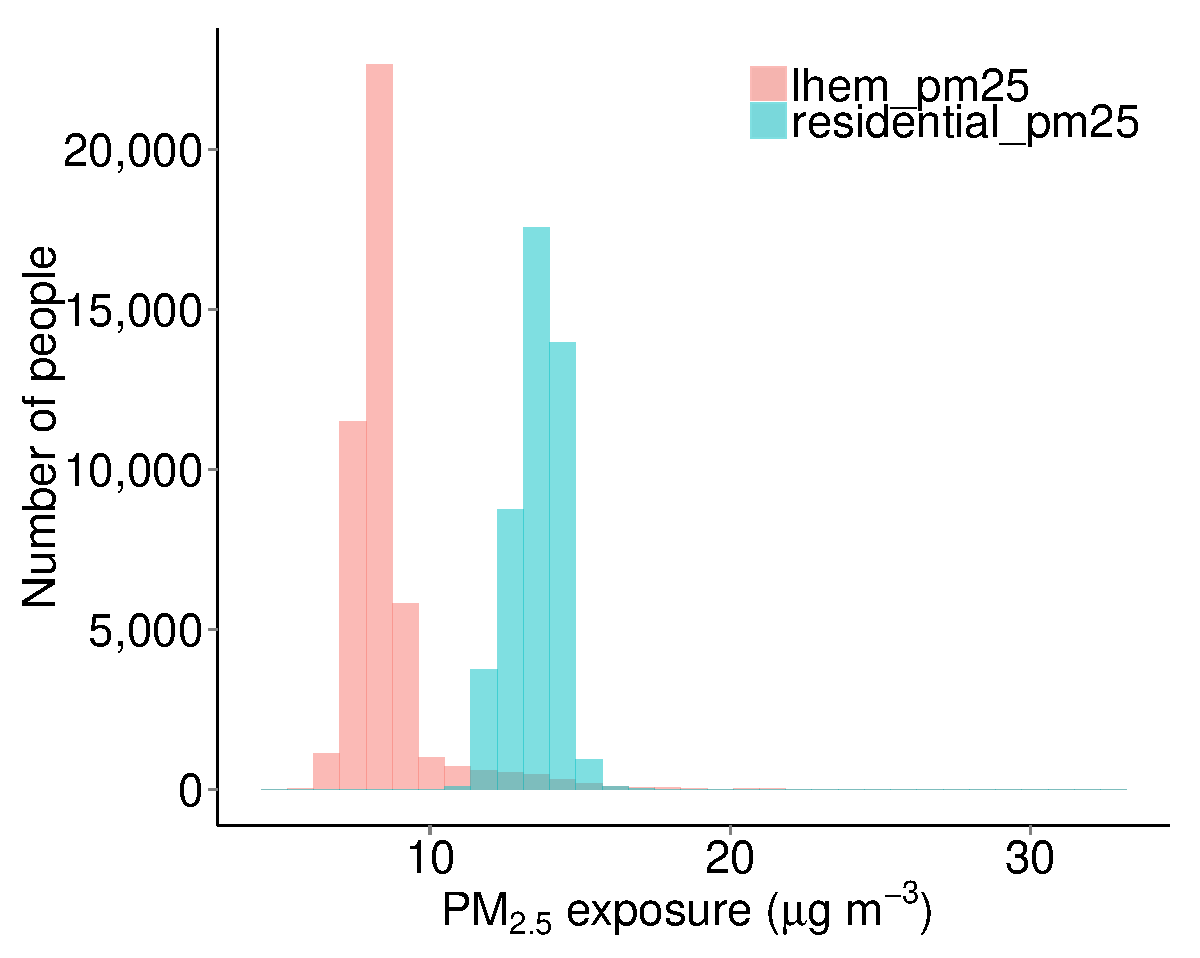
\includegraphics[scale=0.6]{address_point_v_lhem_pm25_hist}
\caption{Daily mean exposure to PM$_{2.5}$ comparing address-point exposure with the LHEM}
\label{fig:address_point_v_lhem_pm25_hist}
\end{figure}

Using the LHEM model the exposure of the population is found to be generally lower than estimates based on the residential address. For NO$_{X}$ the LHEM mean is 18.39 $\mu \text{g m}^{-3}$ and the median is 17.03 $\mu \text{g m}^{-3}$, compared to NO$_{X}$ at the residential address of 46.49 $\mu \text{g m}^{-3}$ and 46.05 $\mu \text{g m}^{-3}$ respectively.

For PM$_{2.5}$ the LHEM mean is 8.49 $\mu \text{g m}^{-3}$ and the median is 8.23 $\mu \text{g m}^{-3}$, compared to PM$_{2.5}$ at the residential address of 13.53 $\mu \text{g m}^{-3}$ and 13.62 $\mu \text{g m}^{-3}$ respectively.

In addition to the LHEM finding different mean and medians to address based exposure estimates, we also find different ranges.

The 10th to 90th percentile range for NO$_{X}$ using the LHEM is 11.64 $\mu \text{g m}^{-3}$ to 26.26 $\mu \text{g m}^{-3}$ (a range of 14.62 $\mu \text{g m}^{-3}$), compared to similar percentile ranges for NO$_{X}$ at the residential address of 32.59 $\mu \text{g m}^{-3}$ to 58.69 $\mu \text{g m}^{-3}$ (a range of 26.1 $\mu \text{g m}^{-3}$). That is, we find a smaller range of exposures to NO$_{X}$ using the LHEM than using residential address methods. 

For PM$_{2.5}$ the LHEM has a 10th to 90th percentile range of 7.32 $\mu \text{g m}^{-3}$ to 9.4 $\mu \text{g m}^{-3}$ (a range of 2.08 $\mu \text{g m}^{-3}$), compared to similar percentile ranges for PM$_{2.5}$ at the residential address of 12.32 $\mu \text{g m}^{-3}$ to 14.47 $\mu \text{g m}^{-3}$ (a range of 2.15 $\mu \text{g m}^{-3}$). In brief, the range for PM$_{2.5}$ between the LHEM and address-point is similar.

In figures X and Y the exposure differences between the LHEM and address-point methods are explored by hour of the day.